%!TEX root = Thesis.tex

  \section{Performance Space Exploration with Parallel Genetic Algorithm}\label{sec:pga}
    
    \begin{figure}[t]
      \centering
      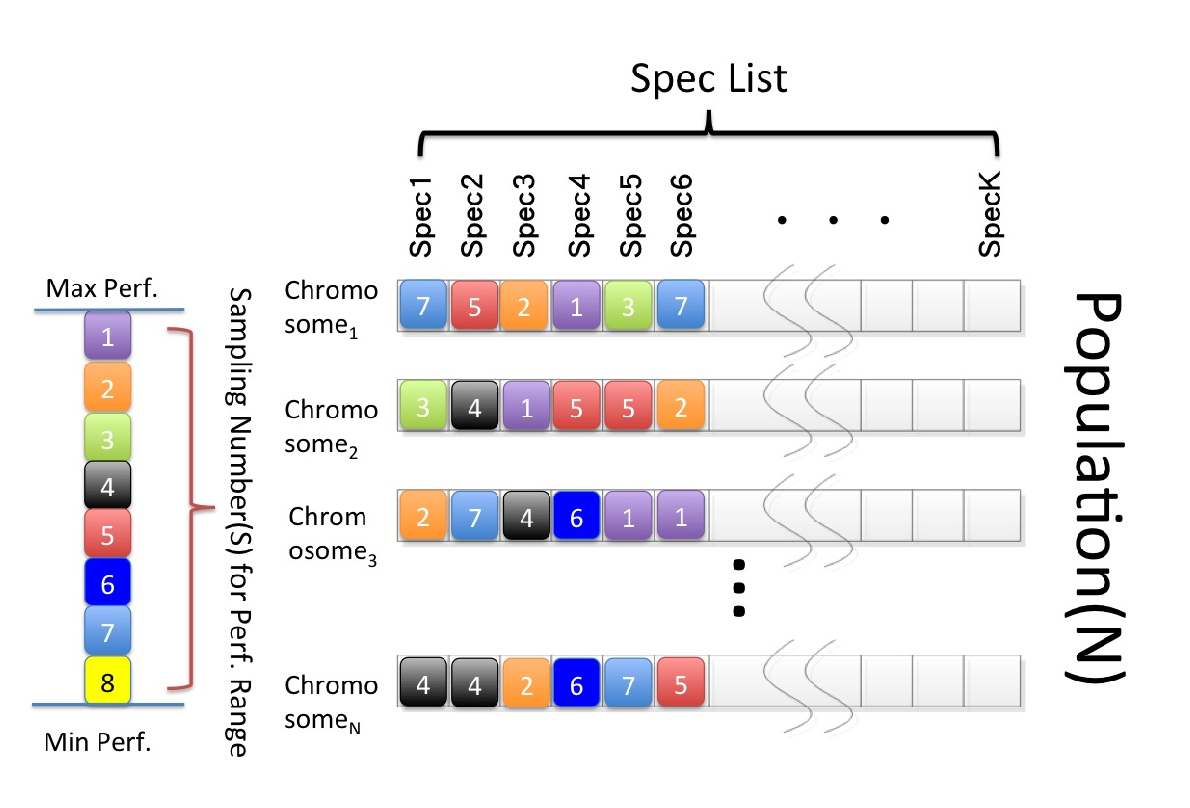
\includegraphics[width=\textwidth]{Fig/Gene.eps}
      \caption{Demonstration of genetic representation for performance metrics.} 
      \label{fig:Gene}
    \end{figure}

    To traverse the space of required circuit performance, we propose an efficient exploration process to investigate the feasible performance metrics of such analog design. Once the set of circuit-level design variables $V^C$ are prepared, these variables can be adopted as parameters into circuit design equations. A set of design equations along with circuit-level parameters, parasitic effects and fitting parameters are constrained with performance requirement. Note that the parasitic effects of the devices are included so as to explore the trade-off between each aspect of performance metrics and circuit-level design variables. To figure out the design equation set with performance constraints is feasible or not, we apply convex optimization. Since the circuit design equations are formulated as geometric programming by posynomial forms, the optimization to find feasible solution with performance constraints is convex. Moreover, to extend the problem with different performance specifications, that each combination of performance constraints can be checked is feasible or not. A set of specification are swept as the constraints for an optimization performance to get performance metrics.
 
    An optimization problem in Eq.(\ref{eq:DesignEq}) describes a unit performance optimization step.

    \begin{align}\label{eq:DesignEq}
      \begin{array}{ll}
      Variables:  & \begin{array}[t]{ll}
                        V^C & = \{{v_k}^C | 1 \leq k \leq |V^C|\} \\
                        V^P   & = \{ v^p_k | 1 \leq k \leq |V^P| \}\\
                        F   & = \{ f_k | 1 \leq k \leq |F| \}\\
                        R   & = \{ r_k | 1 \leq k \leq |R| \} 
                    \end{array}                 \\
        minimize  &   f_{OBJ}( {v_i}^C,v^p_k,f_k)         \\
      subject\ to & \begin{array}[t]{l}
                    r_1 = Perf_1(V^C,V^P,F) \geq z_1\\
                    r_2 = Perf_2(V^C,V^P,F) \geq z_2\\
                    \vdots \\
                    r_k = Perf_k(V^C,P,F) \geq z_k
                \end{array}             
      \end{array}
    \end{align}
    where
    \begin{itemize}
      \item  $V^C$ is circuit level variables extracted from device-level variables.
      \item  $V^P$ is a set of parasitics which is non-ignorable for circuit modeling.
      \item  F demonstrates fitting parameters to fit from circuit-level parameters to performance space.
      \item  R represents the corresponding performance result set which obtain by optimization. 
      \item  $Z = \{z_k| 1 \leq k \leq |Z|\}$ is a set of performance required value. In other words, each $z_k$ represents a value of performance constraint, eg. $z_k \geq 40 \to Av \geq  40dB$
    \end{itemize}
    \vspace{0.3cm}

  
    In every optimization process, one performance metric results in a set of performance metric ($r_1 ,\ldots, r_k$) corresponding to the given specification of performance($z_1,\ldots,z_k$). Therefore, according to the same design equation for optimization, it is an one to one mapping relationship from spec to result of performance and the corresponding circuit-level design variables. 

    To extend the optimization range. Each $z_k$ can be varied with a range of value, that is, we define a maximum value of $z_{kMAX}$ and one minimum value of $z_{kmin}$ with several step value between them. Therefore, we can investigate the performance limitation for $z_k$ by implementing optimization on a series of $z_k$, $z_k=\{z_{ki}| 1 \leq i \leq |z_k|, z_{kMAX} \leq z_{ki} \leq z_{kmin} \}$. Obviously, a set of different performance types with a range of such values are similar to chromosome concept in heredity. As we can see in Fig.~\ref{fig:Gene}, if every chromosome carries different value of every performance metric $z_k$. An evolutionary computing with genetic algorithm for traversing solution space can be employed for traversing optimized multi-objective problem. As mentioned in Section~\ref{sec:PGAIntro}, we further utilize the {\it Parallel Genetic Algorithm} to develop with. The detail implementation is as follows:

    


    \subsection{PGA Overview}

      The methodology to exercise PGA fusion with performance exploration is shown in Algorithm~\ref{alg:PGA}. PGA traverses the performance space by evolution. According to \cite{SurveyDistPGA1997}, our approach picks the coarse-grained fashion PGA. In traditional genetic algorithm, one major population has numbers of individual chromosomes for evolution. In coarse-grained genetic algorithm, the major population is separated into numbers of sub-populations with the same size of individual. Since each sub-population contains large number of individuals, it is time-consuming to exercise fine-grained structure. Therefore, the coarse-grained structure is much efficient at this situation. 


      \begin{figure}[t]
        \centering
        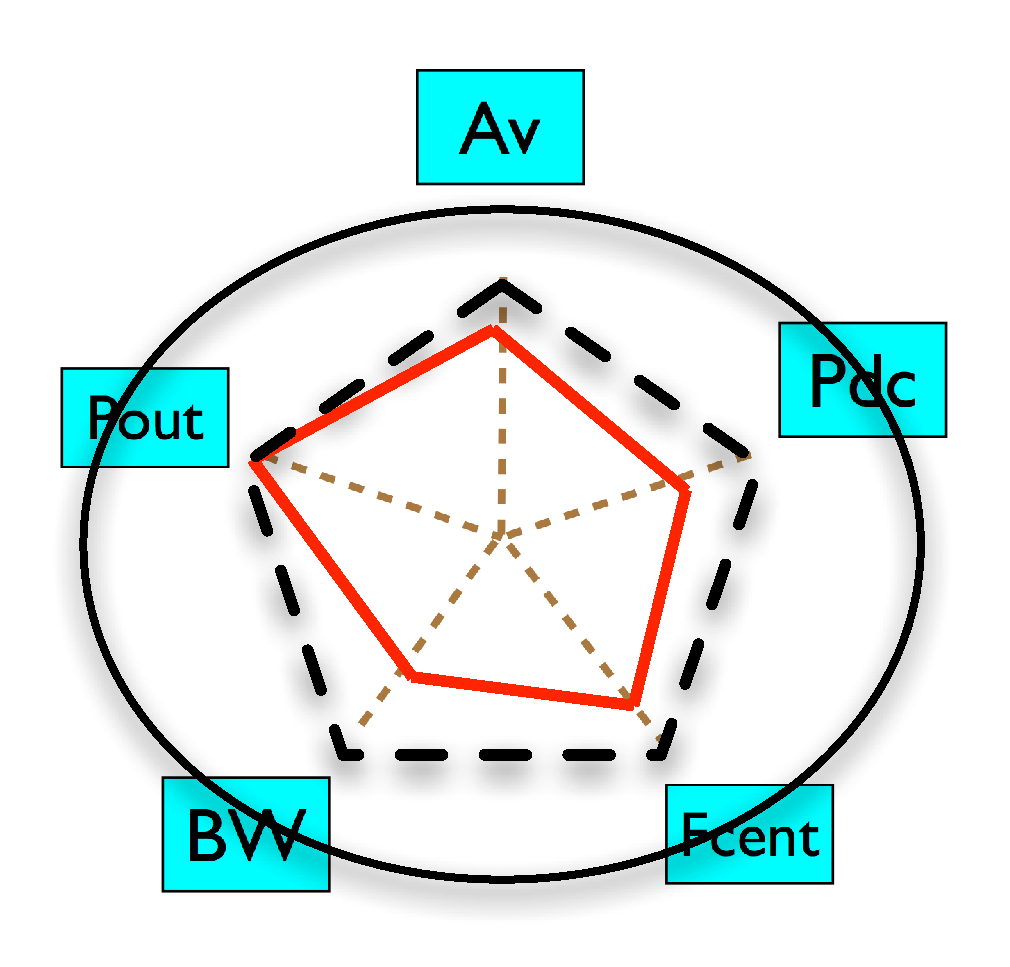
\includegraphics[width=\textwidth]{Fig/MultiSpec.eps}
        \caption{Illustration of performance characteristic (e.g., Av, Pdc, Pout, BW, Fcent, etc.) for each circuit.} 
        \label{fig:MultiSpec}
      \end{figure}


      \newcommand{\PGA}{\ensuremath{\mbox{\sc PGA}}}
      \algloopdefx{RETURN}[1][]{\textbf{return} #1}
      \algblockdefx{FORALLP}{ENDFAP}[1]%
      {\textbf{for all }#1 \textbf{do in parallel}}%
      {\textbf{end for}}
      \begin{algorithm}[t]  
        \caption{$\PGA(Z_{K\times S},N_P,S,k,T,C,M_P)$}\label{alg:PGA}                       
        \begin{scriptsize}
          \begin{algorithmic}[1]
            \REQUIRE 
              \begin{tabular}{l}
              $Z_{K\times S}$: Performance Space Matrix. \\
              $N_P$: Number of Individuals in major population.\\
              %$N_S$: Number of sub-populations.\\
              S: Sampling number for each performance spec $z_k$\\
              K: Number of Performance spec type\\ 
              T: Technology type. \\
              C: Circuit type.\\
              $M_P$: Migration rate.
                \end{tabular}
            \ENSURE 
              \begin{tabular}{l}
                $R_{K \times S}$ : The result performance space\\
                    $P$ : The population of performance specs after PGA
                  \end{tabular}
              \FOR {$i = 1 \to N_P$}
                \FOR {$j = 1 \to k$}
                  \STATE $G_i \gets RandGetSpec(Z_{j\times S})$ \COMMENT{Randomly generate spec value from Z}   
                \ENDFOR
                \STATE $P \gets G_i$
              \ENDFOR
              \FOR {$i = 1 \to k$}
                \STATE $P_i \gets Partition(P,i)$
              \ENDFOR
              \WHILE {Convergence criterion satisfied}          
                \FORALLP {$i = 1 \to k$} 
                  \STATE $R_i \gets Evaluate(P_i,T,C)$
                  \STATE ${Pool}_i \gets Reproduction(P_i,Fitness(T,C,i,R_i))$
                  \STATE $P_i \gets Crossover(P_i,{Pool}_i)$
                  \STATE $P_i \gets Mutation(P_i)$
                \ENDFAP   
                \FOR {$i = 1 \to k$} 
                  \STATE $Migration(P_i,exclusive(P,P_i),M_P)$
                \ENDFOR 
              \ENDWHILE
              \STATE $P \gets Merge(P_1,P_2, \ldots, P_{k})$
              \RETURN $P, R_{K \times S}$  
          \end{algorithmic}
          \end{scriptsize} 
      \end{algorithm}

      As for analog performance optimization, which is a multi-objective problem with a Pareto-front as illustrated in Fig.~\ref{fig:MultiSpec}. To find the Pareto-front, each performance target optima should be traverse as well. Therefore, we further use heterogeneous coarse-grained structure for evolution. In other words, every sub-population deals with different objective that performs optima. For example, one sub-population implement performance exploration to evolve population with better voltage gain($A_v$). Therefore, we pick the fitness function which emphasizes on such performance item($A_V$). Moreover, each sub-population has its own fitness function and evolve independently. Additionally, the diversity for the overall population also can be maintain by migration strategy in the end of the performance exploration stage.

    \subsection{Chromosome Encoding}

      Before PGA process, the fundamental chromosome encoding should be defined. For one performance target $z_k$, given performance upper and lower bound, $\{\left [z_{kmin},z_{kMAX} \right]$. There exist a set of discrete $z_{k,s}$ among this boundary, where 
      \begin{defi}\label{def:Z}
        $\forall z_k, \exists z_{k,s} \to z_{k,S} = \{z_{kmin} \leq z_{k,s} \leq z_{kMAX}\}$. As Algorithm~\ref{alg:PGA} mentioned in $Input:$, S denotes the sampling number for each $z_k$. Therefore, $z_{k,s} = \{z_{kmin} + ({z_{kMAX}-z_{kmin}})\times s/S | 1 \leq s \leq S\}$
      \end{defi}

      \begin{align}\label{eq:PerfMatrix}
        \begin{array}{rl}
          Z_{K \times S} & = 
              \left[\begin{array}{cccc}
               z_{11} & z_{12} & \dots  & z_{1S} \\
               z_{21} & z_{22} & \dots  & z_{2S} \\
               \vdots & \vdots & \vdots & \vdots  \\
               z_{K1} & \dots  & \dots  & z_{KS} 
            \end{array}\right]
        \end{array}
      \end{align}
   
      where
      \begin{itemize}
        \item K: the number of performance specification types. (eg: Av, BW,...,etc.)
        \item $\left[Z_{min},Z_{MAX}\right]_{k}$, $k = 1, \ldots, K$ is the $k_{th}$ type specification range of the performance space.
        \item S is the sampling number for each $Z_S$ between ${Z_k}_{min}$ and ${Z_k}_{MAX}$.
        \item  $\forall z_{ki} \in Z_{K \times S}$, if $i= 1$, $z_{ki}= {Z_S}_{min}$ and if $i = S$, $ z_{ki}={Z_S}_{MAX}$
      \end{itemize}

      By Definition~\ref{def:Z}, every $z_{k,s}$ for $z_k$ are selected as constraints for an optimization problem which represents the circuit design equation. Here we expand the performance space as an $S \times N$ matrix in Eq.(\ref{eq:PerfMatrix}). Moreover, each performance spec from constraints is is encoded as chromosome G from maximal to minimal in a set of $G = \{g_k| 1 \leq k \leq K\}$. For example, $g_i \in G$ randomly obtains value of the $k^{th}$ spec from $z_{k,1}$ to $z_{k,S}$.

    \subsection{Initialization}
      As algorithm~\ref{alg:PGA} described in $Input$, a set of performance space matrix $Z_{K \times S}$ is given. First of all, a major population is constructed according to $Z_{K \times S}$. Algorithm~\ref{alg:PGA} Line 1 to Line 6 illustrate the process to assign performance specs as chromosome for each individual of the major population iteratively. For the reason that we want to achieve multi-objective optimization, k sub-populations are generated and evolved independently. Therefore, a major population $P$ is generated. According to the size of sub-population $k$, master processor allocates individuals to each slave processor uniformly as sub-population $P_1 \ldots P_{k}$. 
  
    \subsection{Evolution}

      An evolution is executed between Algorithm~\ref{alg:PGA} Line 10 and Line 20. Because the $Evaluate$, $Reproduction$, $Crossover$ and $Mutation$ parts are independent, the parallel parts can be performed from algorithm~\ref{alg:PGA} Line 11 to Line 16. Hence, in each sub-population, each location of gene in one individual is fed into $Evaluate(P,T,C)$ as target constraints for performance to the design equation(shown in Eq.(\ref{eq:DesignEq})) and a corresponding result $R_i$ is obtained. However, if one combination of performance metrics produces the solution space which is not convex, such individual would be failed by $Evaluate$. Then, a random generated individual replaces and redoes $Evaluate$ again until each chromosome $G$ has obtained its corresponding result $R = \{r_k| 1 \leq k \leq|R| \}$. 
      
      Fig.~\ref{fig:PGAFlow} shows the flow of the parallel genetic evolution from random performance space matrix($Z_{K\times S}$) to convergence. Each sub-population experiences a evolution with $Evaluate$, $Reproduction$, $Crossover$ and $Mutation$. Between algorithm~\ref{alg:PGA} Line 12 to Line 15, parallel genetic algorithm utilizes a fitness function to determine the suitability for each $G_i$. In our algorithm, we use the $Heterogeneous\ Island$ architecture \cite{SurveyCGPGA1994}. According to our requirement, we tend to specialize the particular spec, such as voltage gain($A_v$). A set for fitness function is given, $Fitness = \{{fitness}_i| 1 \leq i \leq k\}$ as kind of objective function to determine how important each individual is with the $Evaluate$ result. Each sub-population $P_i$ applies one particular fitness function which is related to the required performance result $R_k$ of $Evaluate$ value. Therefore, the fitness function determines the qualified individuals to be preserved to the crossover pool in a weighted ratio, and the others should be extinct. In $Crossover$ of algorithm~\ref{alg:PGA} Line 14, the $Crossover$ step selects each two genes $G_i$ and $G_j$ ,where $\{G_i,G_j \in Pool; 1 < i<j<N\} $ for copulation. Since each individual has $K$ types of spec, these two individuals exchange {\bf c} specs and reserve {\bf $K-c$} specs with each other. In the end of parallel sub-level evolution, the {\it Mutation} step picks up one individual with mutation rate and then replaces one gene value by one slot of $Z_K$. 
    
      \begin{figure}[t]
        \centering
        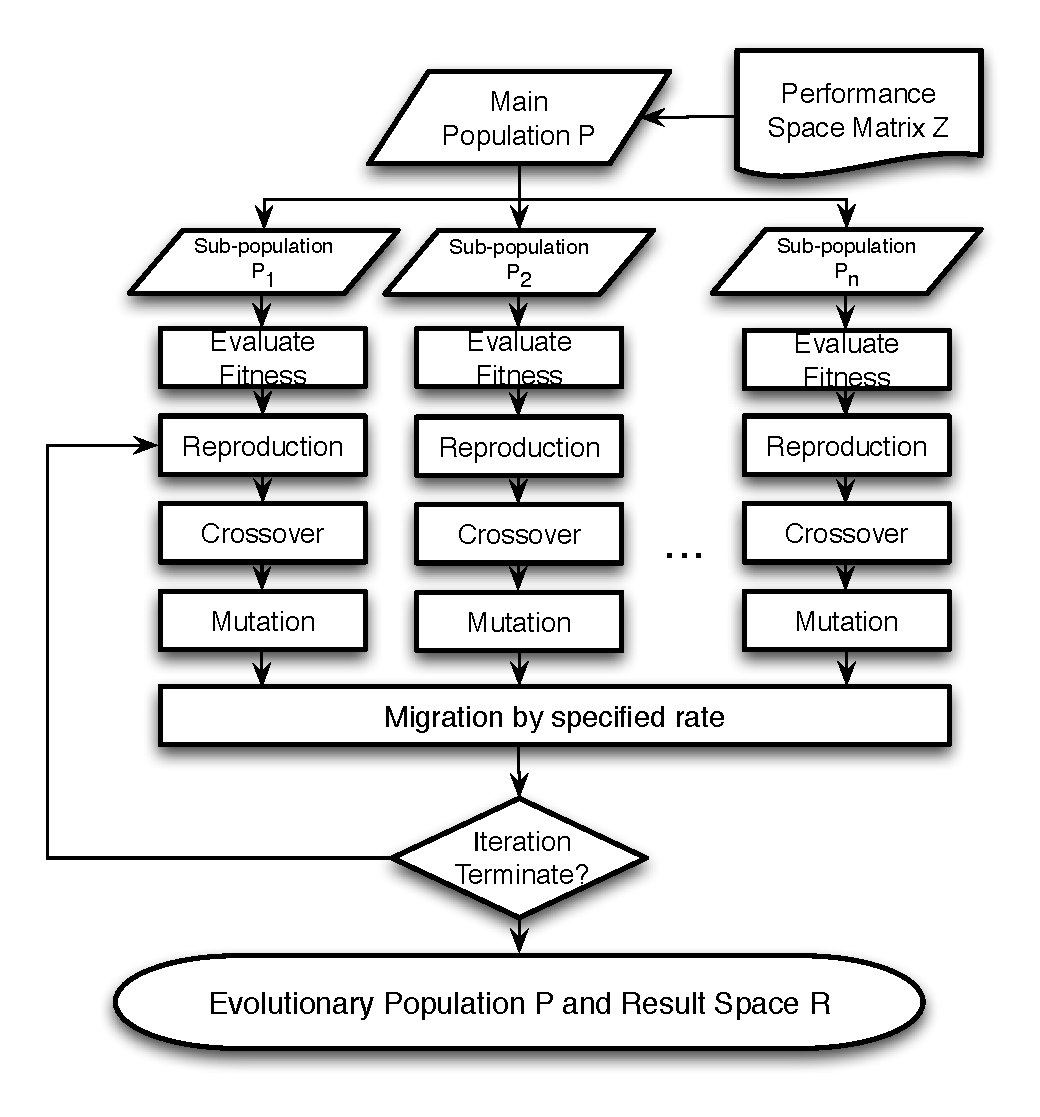
\includegraphics[width=\textwidth]{Fig/PAGEflowchart.eps}
        \caption{Coarse-grained parallel genetic approach from major population P to partitioned population $P_i$ for parallel evolution. The migration step benefits each sub-population on diversity every iteration.} 
        \label{fig:PGAFlow}
      \end{figure}

    \subsection{Migration}  

      \newcommand{\Migration}{\ensuremath{\mbox{\sc Migration}}}
      \algloopdefx{RETURN}[1][]{\textbf{return} #1}
      \algblockdefx{FORALLP}{ENDFAP}[1]%
      {\textbf{for all }#1 \textbf{do in parallel}}%
      {\textbf{end for}}
      \begin{algorithm}[t]  
        \caption{$\Migration(P_i,exclusive(P,Pi),M_P)$}\label{alg:Migration}                       
        \begin{scriptsize}
          \begin{algorithmic}[1]
            \REQUIRE 
              \begin{tabular}{l}
              $P_i$: The population which want to migration, where $i = 1... k$\\
              $exclusive(P,P_i)$: Return a population set except $P_i$ .\\
              %$N_S$: Number of sub-populations.\\
              $M_P$: Migration rate.
                \end{tabular}
            
              \FOR {$j = 1 \to k$}
                  \IF{$j \neq i$}
                    \STATE $R_P \gets rand(0,1)$
            \IF{$R_P \leq M_P$}
                      \STATE  $I_S=bestIndividual(P_i,fitness(T,C,j,R_i))$
              \STATE  $I_R=worstIndividual(P_j,fitness(T,C,j,R_j))$
              \STATE  $replaceIndividual(P_i,P_j,I_S,I_R)$
            \ENDIF
          \ENDIF
                \ENDFOR
             
              \STATE $P \gets Merge(P_1,P_2, \ldots, P_{k})$
              
          \end{algorithmic}
          \end{scriptsize} 
      \end{algorithm}

      In the end of each independent evolution, we perform $Mutation$ with a given mutation rate for sub-population $P_i$ from 1 to $K$. Later, every sub-population is updated. Then, $Migration$ is summarized as shown in Algorithm~\ref{alg:Migration} aims to exchange individuals in the population network shown in the bottom of Fig.~\ref{fig:PGAFlow}. Therefore, each $P_i$ should operate $Migration$ with the others. From algorithm~\ref{alg:Migration} Line 5 to Line 7, each $Migration$ between $P_i$ and $P_j$, $P_i$ exchanges its best individual with respect to ${fitness}_j$, and $P_j$ replaces its worst individual with respect to own ${fitness}_j$ with migration rate $M_P$ in algorithm~\ref{alg:Migration} Line 4. Different sub-population owns its fitness function and uses the particular migration strategy can close to natural evolution. An example of a migration operation between two sub-populations is shown in Fig.~\ref{fig:Migration}. After the $Migration$ is executed, the composition of each $P_i$ is updated with higher diversity. 
    
    \subsubsection{Merge}
      After all, while the termination condition meets, all the sub-populations are generated. These sub-populations not only have good solution with respect to all spec, but also enhance diversity. All individuals in each sub-population merge to a main population one after another. After merge, main population has all the individuals generated from evolution. 
  
  
      \begin{figure}[t]
        \centering
        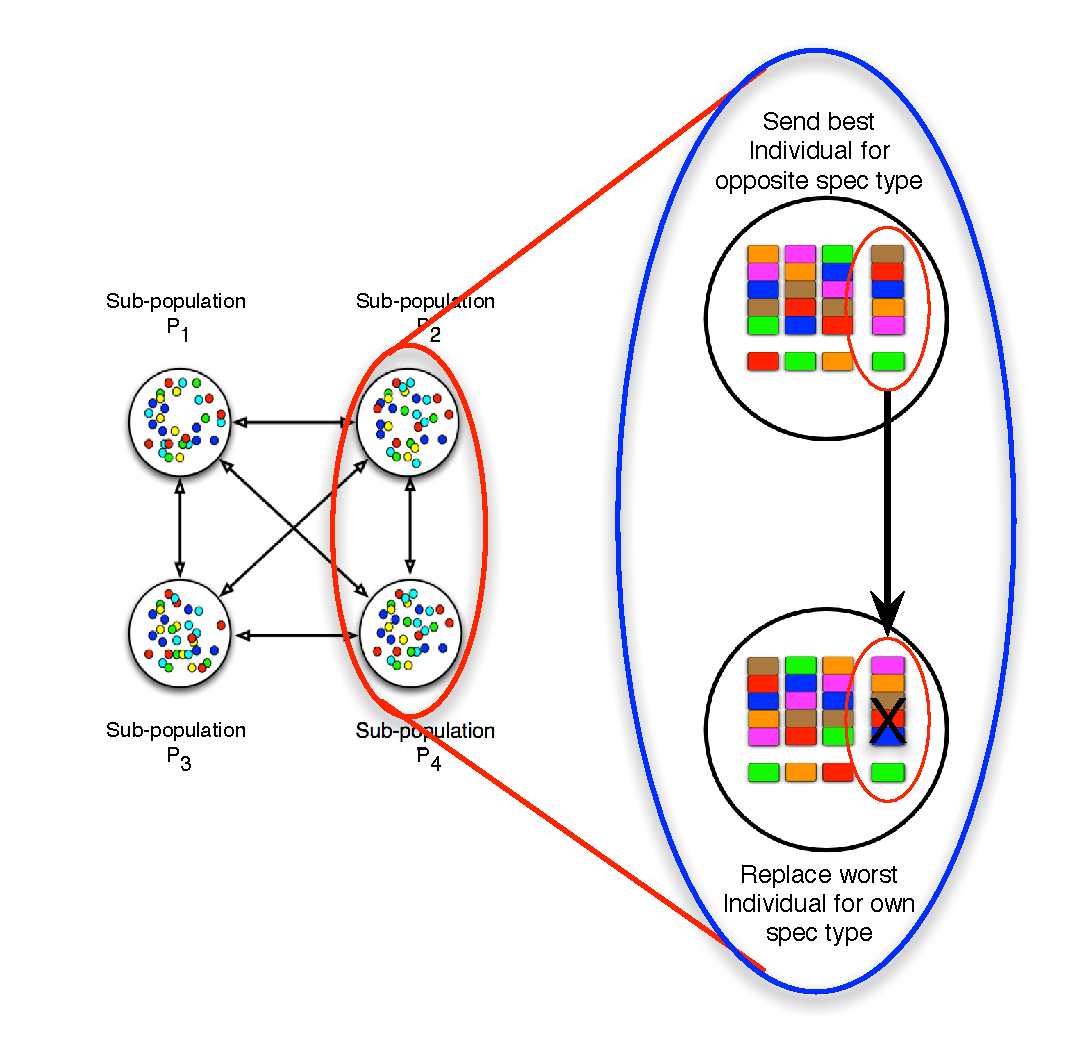
\includegraphics[width=\textwidth]{Fig/PAGEMigration.eps}
        \caption{When sub-population $P_2$ and sub-population $P_4$ perform migration operation with migration rate $M_P$, $P_2$ sends its best individual with respect to spec type $P_4$, and the receiving sub-population $P_4$ replaces its worst individual with respect to its own spec type $P_4$.} 
        \label{fig:Migration}
      \end{figure}

    To consider the complexity of PGA, it is considerable to check the dimension of $Z_{K\times S}$. According to line 12 in Algorithm~\ref{alg:PGA}, $Evaluate(P_i,T,C)$ is the most critical. Each $Evaluate$ for $P_i$ need to resolve $\frac{N_P}{N_S}$ convex optimization problems in serial, which is $O(\frac{N_P}{N_S})$. Comparing to the exhaustive approach, the complexity is restricted to $K$ and $S$. That is, we need to traverse every combination from specification space in $Z_{K\times S}$ for $O(S^K)$ complexity. For example, if a circuit require two performance specs ($A_v$ and $BW$) with 4 sampling steps ($A_v = \{5,10,15,20\}$, $BW = \{3MHz,5MHz,8MHz,10MHz\}$). Therefore, the overall combination of specs need to be checked is $4^2=16$. Obviously, we can observe the gap with more specs($K\uparrow$) and greater precision in sampling($S\uparrow$). To sum up, a genetic-based approach can reduce the complexity by controlling population number and a parallel enhancement further reduce the timing complexity vi parallel number. However, the accuracy is also sacrificed as trade-off.



